\documentclass[12pt]{article}

\usepackage{assignment-texplate}
\usepackage[backend=biber,natbib=true,style=authoryear-icomp,maxnames=3,giveninits=true,uniquename=init]{biblatex}
\usepackage{xurl}
\usepackage{doi}
\bibliography{ref.bib}

\input{limao-preamble}

% ===== CHANGE YOUR DETAILS HERE ============================================= %

\newcommand{\authorName}{Limao Chang}
\newcommand{\assignmentName}{Exploring Thorax and Wing Traits: A Classification Study of Drosophila Species}
\date{May 23, 2024}

% ===== Page title, header, footer setup ===================================== %

\author{\authorName}
\title{\assignmentName}

\pagestyle{fancy}
\fancyhf{}
\lhead{\assignmentName}
\rfoot{Page \thepage}

% ===== Formatting =========================================================== %

% Center title
\renewcommand\maketitlehooka{\null\mbox{}\vfill}
\renewcommand\maketitlehookd{\vfill\null}

\setlength{\headheight}{15pt}  % Vertical height of header




\begin{document}

\begin{titlingpage}
    \maketitle
\end{titlingpage}

\tableofcontents

\newpage
\section{Introduction}

Many datasets on Australian \textit{Drosophila} (fruit fly) species have been collated and studied to investigate questions around climate adaptation, species distribution limits, and population genetics \parencite{datasetcollections}. In this report, we investigate one such dataset \parencite{dataset} which has collected various thorax and wing measurements, and focus on the classification of two such species, \textit{Aldrichi} and \textit{Buzzatii}, based on these traits. 

In the study, the flies were taken from 5 Queensland populations: Binjour, Gogango Creek, Grandhcester, Oxford Downs, and Wahruna. They were kept in the lab for five generations at 25°C, and many thorax and wing measurements were taken on progeny of the fifth generation, which were reared at three temperature treatments (20, 25, and 30°C) \parencite{datasetcollections}. Each measurement was replicated 3 times across 10 different vials.

\section{Exploratory Data Analysis and Cleaning}

\subsection{Exploring the Dataset}

There are $n = 1,731$ measurements and $20$ columns in the original dataset. A summary of the columns is as follows:

\begin{itemize}
    \item The majority of the columns are related to wing and thorax measurements (in mm).
    \item The temperature, vial, and replicate columns are related to the experimental setup of the study, and may or may not be relevant predictors for species classification. The relevance of these features will be investigated in the next subsection.
    \item Since the lab populations were collected in 1994, there is only one \texttt{Year\_start} and \texttt{Year\_end} value for all the measurements, so this feature is redundant.
    \item The population from which each measurement was taken is given in two forms -- the location name, \texttt{Location}, and its geographical coordinates, \texttt{Latitude} and \texttt{Longitude}. These are equivalent, so we choose to ignore the \texttt{Latitude} and \texttt{Longitude} columns, as it is clearer from \texttt{Location} that it is a categorical variable.
\end{itemize}
After cleaning up the columns, there was one invalid value in \texttt{Thorax\_length} and \texttt{wing\_loading}. Both values belonged to the same measurement, so it was removed for the rest of the analysis.

\subsection{Working with Categorical Variables}

Some columns like \texttt{Sex} and \texttt{Population} are categorical variables. For our models, these need to be encoded as numeric values. The easiest way to do this is to use arbitrary integer mappings. However, we avoid doing this, as this can imply ordinal relationships that are not there. For example, if we encoded the five \texttt{Population} names as the integers 1--5, a model may compute a summary statistics like the ``average location'', which would not make much sense.

Instead, we use a one-hot encoding scheme to create binary indicators for each category and to avoid creating false ordinal relationships from categorical variables. For \texttt{Population}, this results in five new binary variables: \texttt{Population\_Binjour}, ..., \texttt{Population\_Wahruna}. Importantly, we also encode the replicate and vial columns in the same way. Even though they are numeric (replicates numbered 1--3 and vials numbered 1--10), these numbers are just arbitrary identifiers -- really, they are just categories that happen to be numbered.

One consideration to be made with this approach is that one-hot encoding can drastically increase the number of columns, especially if each column has many unique values to encode. Here we have encoded the \texttt{Sex}, \texttt{Population}, \texttt{Replicate}, and \texttt{Vial} columns, which have 2, 5, 3, and 10 unique values respectively, so in total we have created
\[
    2 + 5 + 3 + 10 = 20
\]
new columns as a result of the one-hot encoding (16 if we replace the original columns). This is not a significant increase in features, and we will also selectively choose features in the next subsection, so this should not be a concern. Overall, this results in 32 columns (31 of which are features), which is summarised in Table \ref{datasetcolumns} below. Some of the one-hot encoded columns have been omitted for brevity.

\begin{table}[!ht]
\begin{center}
\begin{tabular}{|l|l|l|}
\hline
Column Name                                                                                               & Data type & Description                    \\ \hline \hline
\texttt{Species}                                                                                          & string    & Species name                   \\ \hline
\texttt{Population\_Binjour}, ..., \texttt{Population\_Wahruna}                                           & bool      & Population indicators          \\ \hline
\texttt{Temperature}                                                                                      & int       & Rearing temperature            \\ \hline
\texttt{Vial\_1}, ..., \texttt{Vial\_10}                                                                  & bool      & Vial indicators                \\ \hline
\texttt{Replicate\_1}, ..., \texttt{Replicate\_3}                                                         & bool      & Replicate indicators           \\ \hline
\texttt{Sex\_male}, \texttt{Sex\_female}                                                                  & bool      & Sex indicators                 \\ \hline
\texttt{Thorax\_length}                                                                                   & float     & Thorax length (mm)             \\ \hline
\texttt{l2}, \texttt{l3p}, \texttt{l3d}, \texttt{lpd}, \texttt{l3}, \texttt{w1}, \texttt{w2}, \texttt{w3} & float     & Various wing measurements (mm) \\ \hline
\texttt{wing\_loading}                                                                                    & float     & Wing to thorax ratio           \\ \hline
\end{tabular}
\end{center}
\caption{Cleaned Dataset Columns}
\label{datasetcolumns}
\end{table}

\subsection{Feature Selection using Mean Decrease in Impurity (MDI)}

Feature selection is the idea of selecting only the most relevant features for the task, while discarding redundant or inconsistent features. This can be crucial for datasets with a large number of rows and/or a large number of features (particularly if $n_{\text{features}} \gg n_{\text{rows}}$), because more features leads to more computation and a more complex model. Given two models with comparable predictive performance on the training data, we would in general prefer the simpler model, as it is less likely to overfit to unseen data (this corresponds to a lower model variance in the bias-variance tradeoff).

The dataset here is not too large, but it can still be useful to do some feature importance analysis, e.g. for interpretability of the data and results. Here we will train a random forest classifier\footnote{Later we will also use a random forest model for classification, but here we train it only for the purpose of feature selection.} on the training data, and rank features by their \textit{mean decrease in impurity} (MDI).

In a decision tree, the \textit{purity} of a node measures how ``mixed'' the data points within are, with respect to their classes. A node is 100\% pure if all its data points belong to one class. One of the most common measures of purity is \textit{Gini impurity}, which is a measure of how well the decision tree's misclassification rate improves as compared to a random labelling scheme based on the distribution of classes in the data. The mean decrease in impurity for a feature then calculates how much the feature contributes to decreasing the impurity in each tree in the ensemble, weighted by the number of samples in each node, and then averaged across all the trees in the ensemble \parencite{mdi}.

In short, the idea is that \textbf{features that are more effective at distinguishing between classes will lead to larger reductions in impurity when they are used as decision nodes, and so are more important}. 

\begin{figure}[ht]
\begin{center}
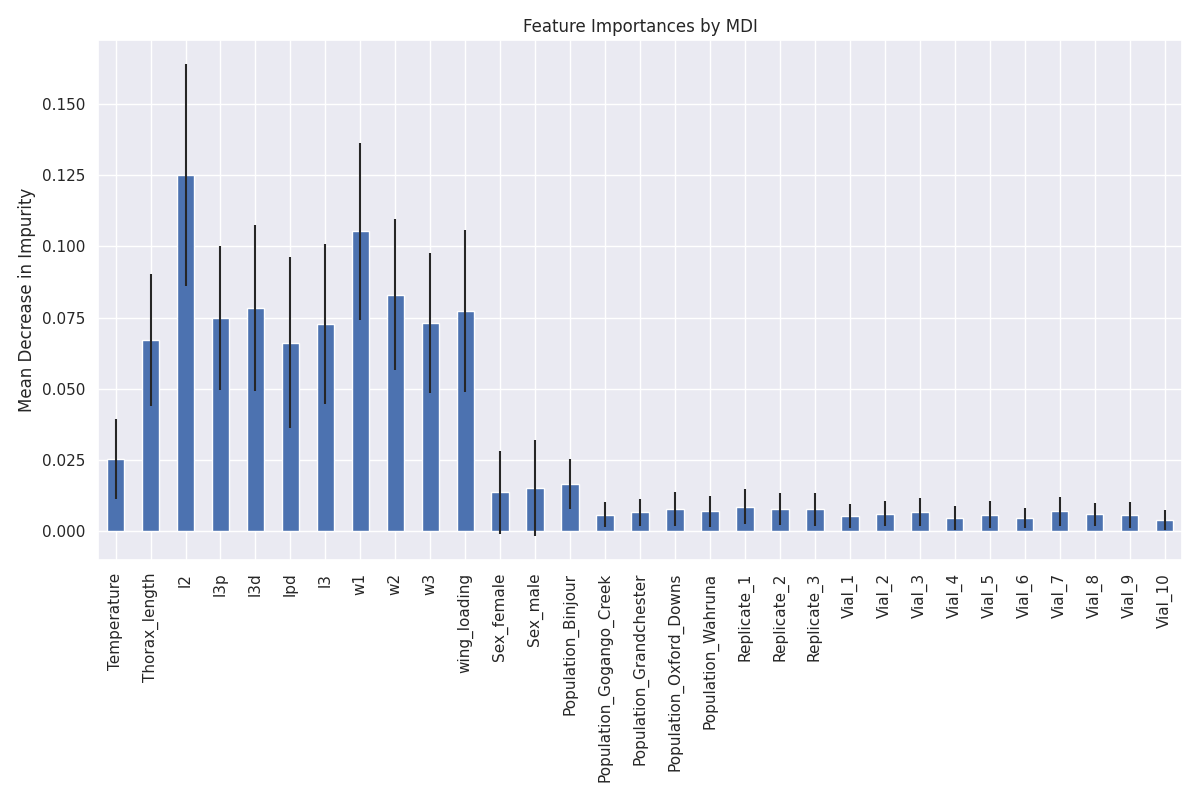
\includegraphics[width=0.9\textwidth]{fig/mdi_feature_importances.png}
\end{center}
\caption{Feature Importances by Mean Decrease in Impurity (MDI)}
\label{featureimportancesmdi}
\end{figure}

Using this metric for feature importance, we can get an idea of how important each predictor is. Figure \ref{featureimportancesmdi} shows the mean decrease in impurity for each of the 31 predictors in the dataset, with the standard deviation across the trees in the ensemble (of which there were 100) overlayed as black bars. In summary, we are left with 14 columns (13 predictors) after the feature selection process.

\begin{itemize}
    \item The variables corresponding to the wing and thorax measurements are by far the most important predictors of species classification, which is to be expected.
    \item The sex and \texttt{Temperature} variables are somewhat important, so we will leave these in the dataset. However, as there are two sex categories, we can remove one (an indicator for one tells us what the indicator for the other will be).
    \item The replicate and vial variables have relatively small MDI values, and so are not important predictors. To save on computational efforts and model complexity, we will remove these columns.
    \item While most of the population variables have insignificant MDI values, \texttt{Population\_Binjour} is a somewhat significant predictor. This indicates that perhaps knowing that a fruit fly comes from Binjour can be a distinguishing feature, but not so for any of the other locations. As such, we remove all of the population variables except for \texttt{Population\_Binjour}.
\end{itemize}


% \subsection{Principal Component Analysis (PCA)}
% 
% PCA is a technique used to reduce the dimensionality of a dataset in such a way that the variance structure is largely preserved. Specifically, we find the $k$ \textit{principal components} (where $k$ is a user-chosen value) such that, when the data is projected down into this $k$-dimensional space, the largest amount of variance in the original data is captured.

\section{Model Selection}

In this section, we explore the use of several models for the species classification problem, and evaluate their results on a test dataset. 70\% of the data was used for training (the same data as was used for feature selection), and 30\% for testing.

\subsection{Logistic Regression}

A logistic regression classifier is like a linear regression model, but applies a sigmoid to the output to constrain its range to $[0,1]$. For the two-class classification problem, the classifier will simply pick the class corresponding to the highest probability.

\subsubsection{Training}

The main consideration for logistic regression is whether we choose to apply regularisation when training, and if so, which regularisation scheme we choose.

Regularisation is a technique used to prevent overfitting by penalising large coefficients to keep them small. For a logistic regression model, the most common choices are the $L_1$ penalty term and the $L_2$ penalty term. The main difference is that $L_1$ regularisation tends to result in sparse solutions; that is, it is more likely to set particular coefficients to zero. This can be viewed as a sort of feature selection, and can so be helpful for interpretability. The $L_2$ penalty penalises larger coefficients more heavily than it does smaller ones, so it tends to result in solutions with smaller (but not zero) coefficients on average.

We will refer to the three models as the ``no-reg'' model, the $L_1$ model, and the $L_2$ model. To select the optimal value of $\lambda$ for the $L_1$ and $L_2$ models, we perform stratified 5-fold cross validation (which ensures the folds have roughly the same proportion of species types). Figure \ref{logreggridsearchcv} displays the cross validation mean accuracy scores for a range of $\lambda$ values for both the $L_1$ and $L_2$ models. For the $L_1$ model, the optimal value was $\lambda = 0.2$, and for the $L_2$ model, the optimal value was $\lambda = 0.1$. Interestingly, the mean accuracy score decreases as the regularisation strength $\lambda$ increases for both models. This suggests that this problem may not require much (if any) regularisation at all.

\begin{figure}[!ht]
\begin{center}
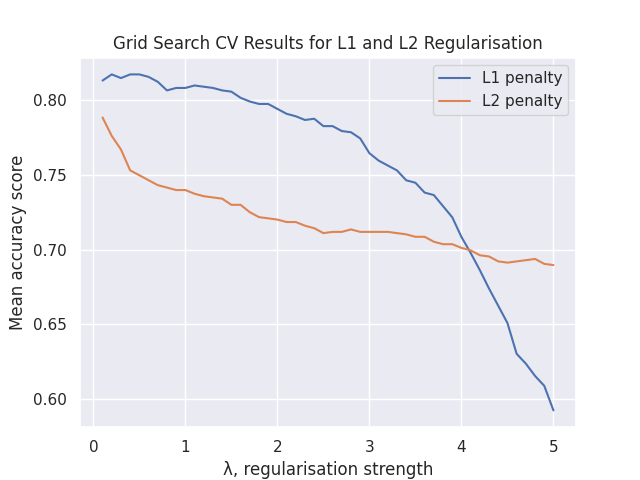
\includegraphics[width=0.6\textwidth]{fig/grid_search_cv_l1_l2_logreg.png}
\end{center}
\caption{Grid Search Cross Validation Results for $L_1$ and $L_2$ Penalty Models}
\label{logreggridsearchcv}
\end{figure}

\begin{figure}[!ht]
\begin{center}
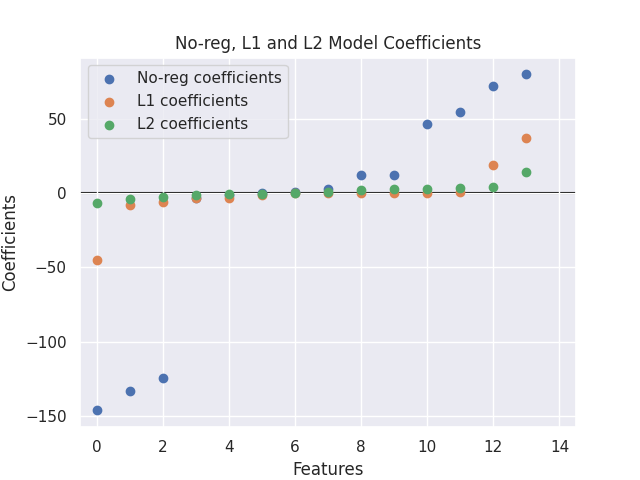
\includegraphics[width=0.6\textwidth]{fig/coef_logreg.png}
\end{center}
\caption{Sorted Coefficients of Logistic Regression Models}
\label{logregcoef}
\end{figure}

The (sorted) feature coefficients after training for each model are given in Figure \ref{logregcoef}. As expected, the unregularised model has larger (in magnitude) coefficients than the regularised models. The $L_2$ model penalises large coefficients, so it has comparatively small (in magnitude) coefficients. It is a bit difficult to tell from the graph, but the $L_1$ model has zeroed the coefficients corresponding to the \texttt{l3p}, \texttt{lpd}, \texttt{l3}, and \texttt{w3} features, which are all wing measurements. In comparison, neither the no-reg nor the $L_2$ model had any zero coefficients.

\subsubsection{Results and Discussion}

The results are tabulated in Table \ref{logregperformance}. The no-reg model and the $L_1$ model perform very similarly on the training set, with each model attaining around 82\% training accuracy. The $L_2$ model performs slightly worse, attaining around 78\% training accuracy. Interestingly, we note that the no-reg model performs the best on both the training and test datasets. That being said, the differences between the no-reg and $L_1$ models are quite small ($<$1\% difference in both the training and test accuracy). The $L_2$ model however does perform noticeably worse than the other two.

This does corroborate with what we found in Figure \ref{logreggridsearchcv} -- which is that the mean accuracy score tended to get worse as regularisation strength increased, so indeed it is likely that this problem does not require regularisation.

\begin{table}[!ht]
\begin{center}
\begin{tabular}{|c|c|c|c|}
\hline
Model             & No-reg & $L_1$ & $L_2$ \\ \hline
Training accuracy & 0.824  & 0.822 & 0.784 \\ \hline
Test accuracy     & 0.794  & 0.784 & 0.751 \\ \hline
\end{tabular}
\end{center}
\caption{Performance of Logistic Regression Models}
\label{logregperformance}
\end{table}

The confusion matrices (on the test dataset) for all three models are given in Figure \ref{logregcm}. The no-reg and $L_1$ models specifically have a very similar number of correct and incorrect classifications for each species type.

\begin{figure}[!ht]
\begin{center}
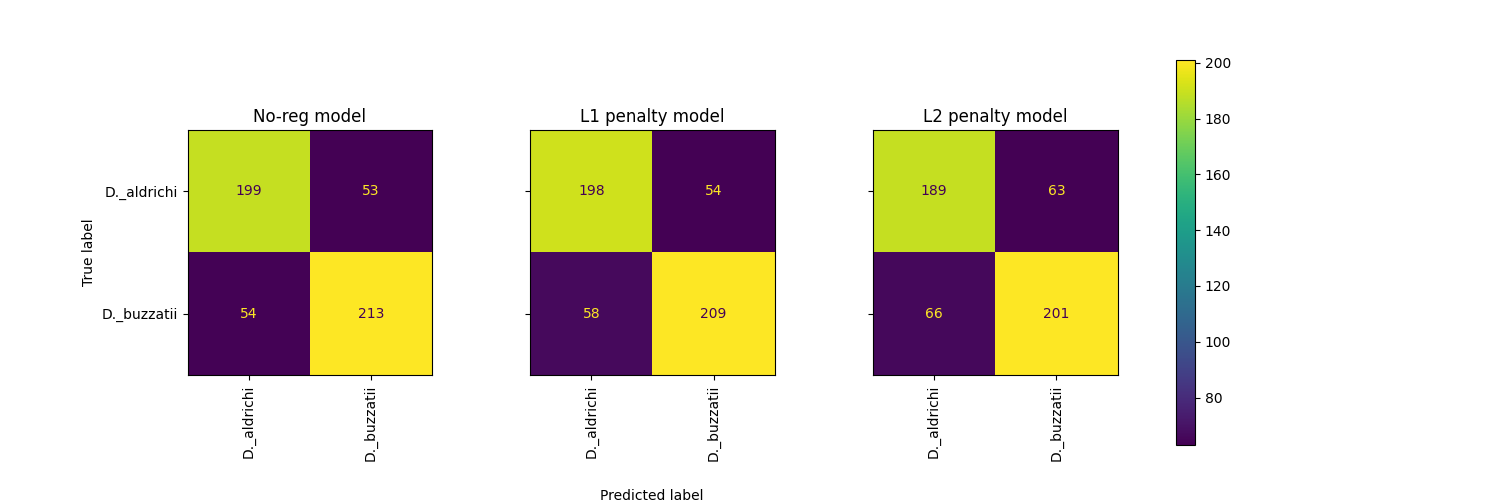
\includegraphics[width=\textwidth]{fig/cm_logreg.png}
\end{center}
\caption{Confusion Matrix (test dataset) for Logistic Regression Models}
\label{logregcm}
\end{figure}

\newpage
\subsection{Random Forest}

A random forest is an ensemble model consisting of decision trees. A decision tree can be thought of as a model that predicts the classification (alternatively, the probability distribution of classifications) of a given input by answering a series of yes-no questions about the input. Each question is a decision node in the tree. A random forest's prediction is then the one with the highest mean probability across all its trees.

Usually, each tree is trained on bootstrap samples of the dataset, which creates variation in the learned trees. Random forests also employ a technique to further decrease the correlation between trees, which is to only allow each tree to consider a random subset of predictors when training and creating the decision nodes.

\subsubsection{Training}

During training, there are two important hyperparameters that we need to consider -- the maximum depth of each tree in the forest, and the number of trees in the forest (i.e. the ensemble size).

For the former, we can use cross-validation to select the optimal depth for each of the trees.

\begin{figure}[!ht]
\begin{center}
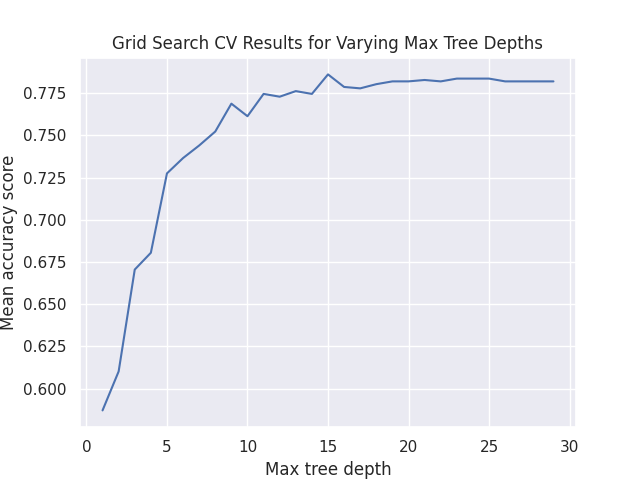
\includegraphics[width=0.6\textwidth]{fig/grid_search_cv_random_forest.png}
\end{center}
\caption{Grid Search Cross Validation Results for Varying Tree Depths}
\label{randomforestgridsearchcv}
\end{figure}

Figure \ref{randomforestgridsearchcv} displays the cross validation mean accuracy scores for a range of max tree depths. As the max tree depth increases, the CV score also tends to increase. This is maximised at a depth of 15, which we will pick for our final classifier, as it is conveniently also a good balance between high CV score and relatively low model complexity. For the sake of comparison, we will also train a random forest classifier with a depth of 5, which will be a much simpler model.

\begin{figure}[!ht]
\begin{center}
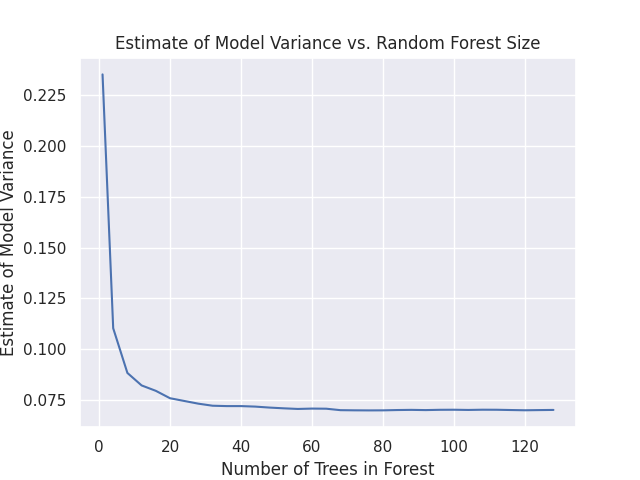
\includegraphics[width=0.6\textwidth]{fig/model_variance_random_forest.png}
\end{center}
\caption{Estimate of Model Variance vs. Random Forest Size}
\label{randomforestvariance}
\end{figure}

For the latter hyperparameter (ensemble size), it can be shown that adding more ensemble members to the model reduces the model variance\footnote{the model variance is still limited by the average correlation between the trees.} without increasing the model bias \parencite{smlbook}. This means that having a larger number of trees in the forest does not lead to overfitting, so the main motivation for choosing a smaller number of trees is the computational cost (as each tree needs to be fit during training).

To pick an optimal number of trees, we estimate the model variance for the random forest classifier with varying numbers of trees. The results are given in Figure \ref{randomforestvariance}. As expected, the model variance tends to decrease as the number of ensemble members increases until it eventually plateaus. For our random forest classifiers, we will pick an ensemble of 40, as it is roughly where the variance plateaus, and so there is little benefit in picking a larger forest.

\subsubsection{Results and Discussion}

The results are tabulated in Table \ref{randomforestperformance}. Two random forest classifiers were trained on the training dataset -- one with a max tree depth of 5 and one with 15. Both classifiers were trained with 40 trees in the forest. We can see from the results that both random forest classifiers exhibit similar behaviour: they performed relatively well on the training dataset but noticeably worse on the test dataset. This suggests that both models are possibly overfitting to the training data. This is almost certainly the case for the 15-depth model, as it has near perfect accuracy on the training set, but 22\% less accuracy on the test dataset.

\begin{table}[!ht]
\begin{center}
\begin{tabular}{|c|c|c|c|}
\hline
Model             & max\_depth=5 & max\_depth=15 \\ \hline
Training accuracy & 0.822  & 0.998 \\ \hline
Test accuracy     & 0.709  & 0.778 \\ \hline
\end{tabular}
\end{center}
\caption{Performance of Random Forest Models}
\label{randomforestperformance}
\end{table}

The confusion matrices for both random forest models are given in Figure \ref{randomforestcm}. Both models correctly classified roughly the same number of \textit{buzzatii} species, but the 15-depth model correctly classifies more \textit{aldrichi} species. It appears that the 5-depth model struggles most with classifying measurements whose true species type is \texttt{aldrichi} (as it only correctly classifies $\approx 63\%$ of these).

\begin{figure}[!ht]
\begin{center}
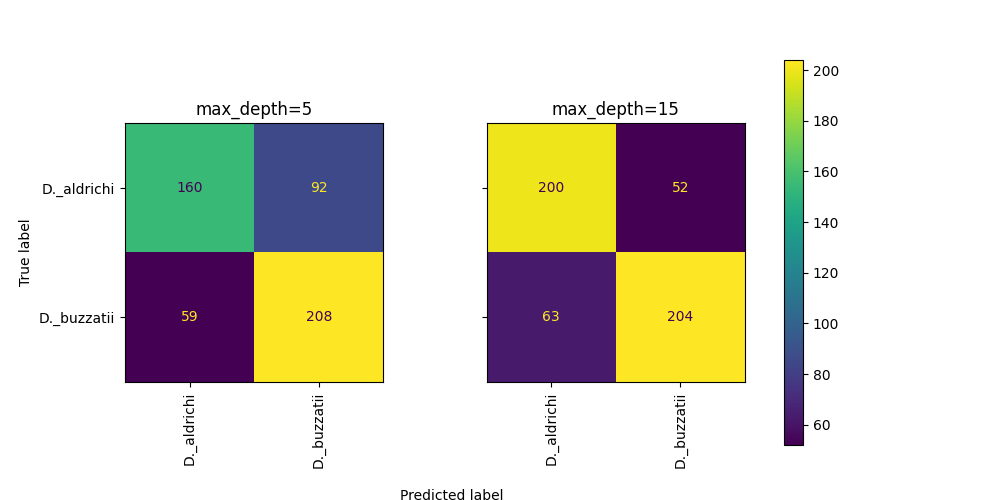
\includegraphics[width=\textwidth]{fig/cm_random_forest.png}
\end{center}
\caption{Confusion Matrix (test dataset) for Random Forest Models}
\label{randomforestcm}
\end{figure}

\subsection{Support Vector Machine (SVM)}

A support vector machine (SVM) for the two-class classification problem aims to find a hyperplane in the feature space that best separates the data points. This is, intuitively, the hyperplane that has the largest margin between the two classes, that is, the hyperplane such that the distance to the nearest data point for each class is maximised \parencite{smlbook}. In the case where the data is not linearly separable, the original feature space can be transformed into a higher-dimensional feature space where it may be easier to linearly separate the data \parencite{svmkernel}. This is essentially what we do when we make the choice of kernel in an SVM.

\subsubsection{Training}

For a SVM, a key consideration is the kernel type that is used, which affects the notion of similarity between data points and thus the shape of the decision boundary in the trained classifier. Another consideration is the regularisation strength $\lambda$. For this problem, we consider two choices of kernel: a Gaussian or radial basis function (RBF) kernel, and a polynomial kernel. The Gaussian kernel uses Euclidean distance as a notion of similarity, whereas the polynomial kernel uses cosine similarity on polynomial transformations of the data. Given that these kernels involve computing distances, a standardisation step was taken here to normalise each of the features before feeding it to the SVM.

Figure \ref{svmgridsearchcv} shows the results of grid search CV for varying regularisation strengths and for the two kernels mentioned above, RBF and polynomial (with varying degrees). The effect of regularisation strength is similar to what was observed with the logistic regression model -- stronger regularisation tends to be correlated with weaker CV performance. The RBF kernel and degree-1 polynomial\footnote{Note that this differs slightly from a linear kernel in the \texttt{scikit-learn} implementation: the degree-1 polynomial kernel has an additional bias parameter. For this reason we will continue to refer to it as a polynomial kernel.} kernel performed the best, with the higher degree polynomials performing considerably worse. For both the RBF and degree-1 polynomial, the optimal regularisation value was $\lambda = 0.2$.

\begin{figure}[!ht]
\begin{center}
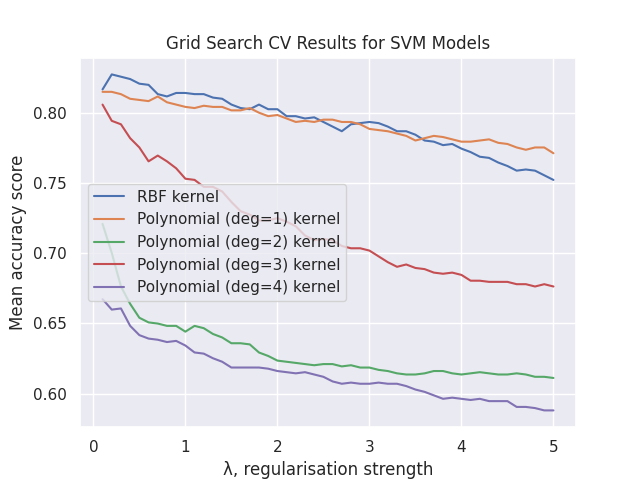
\includegraphics[width=0.6\textwidth]{fig/grid_search_cv_svm.png}
\end{center}
\caption{Grid Search CV Results for Varying SVM Kernels and Regularisation Strength $\lambda$}
\label{svmgridsearchcv}
\end{figure}

It is interesting that the RBF kernel performs just as well as the degree-1 polynomial kernel, since the degree-1 polynomial kernel has a linear decision boundary, whereas the RBF kernel (and the higher-degree polynomial kernels also) has a non-linear decision boundary. Although it is not possible to visualise the decision boundary without e.g. dimensionality reduction of the feature space, we know in the 2-dimensional case, the decision boundaries tend to contract around data points that are close to each other \parencite{svmvis}, so one possible reason for the good performance during CV is the flexibility of the model.

\subsubsection{Results}

The results are tabulated in table \ref{svmperformance}. We can see that the SVM with the RBF kernel performed better across both the training and test datasets. However, the RBF kernel model seems to have overfit slightly to the training set and moreso than the degree-1 kernel model, which is as expected, given the comments in the previous subsection about the flexibility of the RBF kernel.

\begin{table}[!ht]
\begin{center}
\begin{tabular}{|c|c|c|c|}
\hline
Model             & RBF kernel & Degree-1 polynomial \\ \hline
Training accuracy & 0.886      & 0.824               \\ \hline
Test accuracy     & 0.821      & 0.782               \\ \hline
\end{tabular}
\end{center}
\caption{Performance of SVM Models}
\label{svmperformance}
\end{table}

Figure \ref{svmcm} gives the confusion matrices for both SVM classifiers. Similarly to the previous model comparisons, both SVM classifiers are able to correctly classify roughly the same number of \textit{buzzatii} species measurements, and the main difference between the two is the number of incorrect classifications of measurements that are \textit{aldrichi} flies.

\begin{figure}[!ht]
\begin{center}
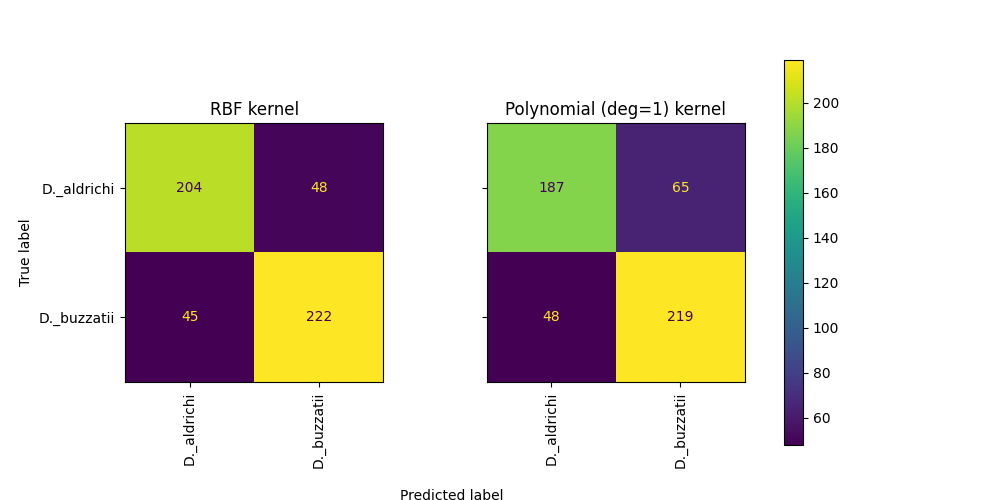
\includegraphics[width=\textwidth]{fig/cm_svm.png}
\end{center}
\caption{Confusion Matrix (test datast) for SVM Models}
\label{svmcm}
\end{figure}

\section{Conclusion}

In this report, we explored the use of several machine learning models to classify the species of a \textit{Drosophila} fruit fly based on various wing and thorax traits. Each of these models were able to provide some insight into the dataset, and performed reasonably well on the classification task, suggesting that the wing and thorax traits of \textit{Drosophila} flies can be a good predictor of the species that a particular fly belongs to.

The SVM classifier with an RBF kernel performed the best on the test dataset, being the only classifier to achieve a test accuracy above 80\%. Many of the other models achieved an accuracy in the high 70\%s, and the logistic regression model with no regularisation in particular did quite well given the simplicity of its decision boundary (which is linear).

As noted in the training and cross-validation of several of the models, greater regularisation tended to result in worse performance. In the case of the logistic regression model, no regularisation yielded the best results on the test dataset. In the case of the SVM, a small regularisation term of $\lambda = 0.2$ yielded the best results on the test dataset. This suggests that little (if any) regularisation is required for this problem, and that the weights learned by the un-regularised models were already quite appropriate in magnitude.

For each model type explored, each variation of the model correctly classified roughly the same number of \textit{buzzatii} species. The main distinguishing factor between the models seems to have been the performance on the \textit{aldrichi} species -- that is, the models with a higher test accuracy tended to correctly classify \textit{aldrichi} species more often. In a sense, this means that the \textit{buzzatii} species was ``easier'' to classify for each of the models in general. This may suggest that there is a stronger relationship between the various wing and thorax measurements collected for the \textit{aldrichi} fruit flies as compared to the \textit{buzzatii} fruit flies.

A further extension of this report could explore the use of more machine learning models. However, the results indicate that a model with a simple linear decision boundary seems to already perform quite well on the dataset, so perhaps a more complex model will not improve much on the performance already seen here. A more practical and potentially insightful extension could be to consider more of the \textit{Drosophila} datasets \parencite{datasetcollections} -- either individually or combined -- to see if other traits of the \textit{Drosophila} can provide more insight into the species.

\clearpage
\printbibliography

\end{document}

